\documentclass[11pt,a4paper]{article}
\usepackage{lmodern}
\usepackage[T1]{fontenc}
\usepackage[utf8]{inputenc}
\usepackage[italian]{babel}
\usepackage[a4paper,margin=2.6cm,headheight=14pt]{geometry}
\usepackage{graphicx}
\usepackage{booktabs}
\usepackage{xcolor}
\usepackage{fancyhdr}
\usepackage{caption}
\usepackage{listings}
\usepackage{microtype}
\usepackage{longtable}
\usepackage[hidelinks]{hyperref}

\definecolor{accent}{HTML}{1F4E8C}
\definecolor{codebg}{HTML}{F4F6F8}
\definecolor{rule}{HTML}{C8D0D8}

\hypersetup{colorlinks=true,linkcolor=accent,urlcolor=accent,citecolor=accent}

\pagestyle{fancy}
\fancyhf{}
\fancyhead[L]{\footnotesize\textsc{OpenTelemetry per workload mixed-criticality}}
\fancyhead[R]{\footnotesize\thepage}
\renewcommand{\headrulewidth}{0.4pt}

\captionsetup{font=small,labelfont={bf,color=accent},width=0.92\textwidth}

\lstset{
  basicstyle=\ttfamily\footnotesize,
  backgroundcolor=\color{codebg},
  frame=leftline, framerule=1.6pt, rulecolor=\color{accent},
  framexleftmargin=6pt, xleftmargin=8pt,
  breaklines=true, breakatwhitespace=false,
  columns=fullflexible, keepspaces=true,
  showstringspaces=false,
  aboveskip=9pt, belowskip=9pt,
  literate={à}{{\`a}}1 {è}{{\`e}}1 {é}{{\'e}}1 {ì}{{\`i}}1 {ò}{{\`o}}1 {ù}{{\`u}}1
           {À}{{\`A}}1 {È}{{\`E}}1 {°}{{\textdegree}}1 {–}{{-}}1 {—}{{---}}1
}

\newcommand{\us}{\,$\mu$s}
\setlength{\parskip}{0.45em}
\setlength{\parindent}{0pt}
\title{\vspace{-1.4cm}\textbf{Valutazione di OpenTelemetry\\per il monitoraggio di workload mixed-criticality}\\[.3em]
\large Campagna sperimentale su Linux PREEMPT-RT}
\author{Benito Cervone \and \textit{(secondo componente del gruppo)}}
\date{\today}

\begin{document}
\maketitle
\thispagestyle{empty}

\begin{center}
\begin{minipage}{0.9\textwidth}
\small\itshape
Questo documento riporta il lavoro svolto per valutare se e in che misura OpenTelemetry sia in
grado di monitorare workload real-time a criticit\`a mista, con particolare attenzione a due
domande: se la pipeline di telemetria sappia \emph{prioritizzare} i task critici rispetto a quelli
best-effort, e quale sia l'\emph{overhead} del monitoraggio sui tempi di risposta. La valutazione
si basa su una campagna di 485 esecuzioni misurate su una piattaforma resa deterministica in modo
controllato. Il codice strumentato \`e stato fornito come base di partenza; il nostro contributo
riguarda la costruzione della piattaforma di misura, il disegno degli esperimenti, la loro
esecuzione e l'analisi dei risultati.
\end{minipage}
\end{center}

\vspace{1em}
{\small\tableofcontents}
\newpage

\section{La piattaforma sperimentale}

Misurare l'overhead di una libreria di tracing significa cercare differenze dell'ordine delle
decine di microsecondi. Su una macchina non preparata, la varianza dovuta a frequenza variabile,
migrazioni di processo e interruzioni \`e di gran lunga superiore al segnale che si vuole
osservare. La prima parte del lavoro \`e stata quindi dedicata a rendere la piattaforma
sufficientemente stabile da rendere significative le misure successive.

\subsection{Hardware e sistema}

Le misure sono state eseguite su un portatile con processore AMD Ryzen 7 3700U (4 core fisici,
8 thread SMT, TDP 15\,W) e kernel Linux \texttt{6.12.79-rt17} con patch PREEMPT-RT, installato
in dual boot su hardware reale e non in virtualizzazione.

Il processore espone 8 CPU logiche appaiate a due a due sui 4 core fisici:

\begin{center}\ttfamily\small
cpu0,\,cpu1 $\rightarrow$ core 0 \quad
cpu2,\,cpu3 $\rightarrow$ core 1 \quad
cpu4,\,cpu5 $\rightarrow$ core 2 \quad
cpu6,\,cpu7 $\rightarrow$ core 3
\end{center}

Tutti i core condividono la stessa cache L3, per cui la scelta di \emph{quali} core utilizzare \`e
indifferente; conta invece che si tratti di core \textbf{interi}. Questo ha determinato due
decisioni.

\textbf{Il task critico e i task di disturbo devono stare su core fisici diversi.} Due thread SMT
dello stesso core condividono unit\`a di esecuzione, cache L1 e L2: collocandoli l\`i,
l'interferenza misurata sarebbe stata in buona parte contesa hardware, cio\`e esattamente il
fenomeno che lo studio deve tenere separato dagli effetti di scheduling e di telemetria. Il task
critico \`e stato quindi assegnato a \texttt{cpu2} (core 1) e i task di disturbo a \texttt{cpu6}
(core 3).

\textbf{Non si isola una CPU lasciando fuori il suo gemello SMT.} Isolando ad esempio le sole
\texttt{cpu2} e \texttt{cpu4}, il carico di sistema che continua a girare sui rispettivi gemelli
sottrarrebbe risorse alle CPU nominalmente isolate, che risulterebbero tali solo sulla carta.
L'isolamento comprende quindi i due core interi: \texttt{2,3,6,7}.

\subsection{Parametri di avvio del kernel}

La riga di comando del kernel \`e stata configurata come segue:

\begin{lstlisting}
isolcpus=managed_irq,domain,2,3,6,7  nohz_full=2,3,6,7
rcu_nocbs=2,3,6,7  irqaffinity=0,1,4,5
\end{lstlisting}

Ciascun parametro risponde a una sorgente di disturbo distinta.

\begin{itemize}
\item \texttt{isolcpus=domain} rimuove le CPU indicate dai domini di bilanciamento dello
scheduler: nessun processo vi viene migrato automaticamente, e vi finisce solo ci\`o che viene
collocato esplicitamente.

\item \texttt{isolcpus=managed\_irq} agisce sul lato di sottomissione delle richieste di I/O: il
livello a code multiple del sottosistema a blocchi non utilizza le code il cui interrupt \`e
associato a una CPU isolata. \`E utile chiarire un equivoco: questo parametro \textbf{non} modifica
l'affinit\`a degli interrupt gestiti dal kernel, che rimane invariata; l'effetto \`e che quelle
code non vengono pi\`u utilizzate, e la verifica corretta \`e quindi il conteggio degli interrupt,
non l'affinit\`a dichiarata. Sulla nostra macchina le code del disco che ricadrebbero sulle CPU
isolate mostrano contatori a zero.

\item \texttt{nohz\_full} elimina il tick periodico di scheduling sulle CPU indicate quando vi
gira un solo task eseguibile. L'effetto \`e stato misurato e non assunto: in 5 secondi di
esecuzione all'interno dell'area isolata si contano \textbf{106} interruzioni di temporizzazione
locale sulla CPU del task critico, contro le 5000 che si avrebbero con il tick pieno alla
frequenza configurata di 1000\,Hz, e contro le 623--1216 osservate sulle CPU di servizio.

\item \texttt{rcu\_nocbs} sposta l'esecuzione dei callback di RCU fuori dalle CPU isolate.

\item \texttt{irqaffinity} fa s\`i che gli interrupt \emph{nascano} affini alle sole CPU di
servizio. Senza questo parametro, alcune periferiche (controller grafico, USB, audio, tastiera)
allocano i propri interrupt sulle CPU isolate, e occorre riassegnarli a posteriori. Dopo la
verifica, tali interrupt risultano affini a \texttt{0-1,4-5} e presentano conteggio nullo sulle
CPU isolate gi\`a prima di attivare l'isolamento a runtime.
\end{itemize}

Restano due categorie non eliminabili, di cui si \`e tenuto conto: i thread di kernel per-CPU
(migrazione, softirq, timer, RCU), che esistono per costruzione su ogni CPU e di cui l'isolamento
riduce l'attivit\`a ma non l'esistenza; e un piccolo numero di interrupt gestiti direttamente dal
kernel, la cui affinit\`a non \`e modificabile ma che, come verificato, non vengono sollecitati.

\subsection{Isolamento a runtime}

Ai parametri di avvio si affianca un isolamento applicato a ogni sessione di misura, che crea due
insiemi di CPU distinti: uno di servizio (\texttt{0,1,4,5}) in cui vengono confinati tutti i
processi esistenti, e uno riservato (\texttt{2,3,6,7}) in cui gira soltanto ci\`o che viene
lanciato esplicitamente. Lo stesso passo riassegna alle CPU di servizio le affinit\`a degli
interrupt che un driver avesse eventualmente allocato altrove dopo l'avvio.

L'efficacia \`e stata verificata sperimentalmente confrontando lo stesso carico dentro e fuori
l'area isolata. Il jitter del periodo, definito come differenza fra periodo massimo e mediano,
passa da 1420--2418\us{} all'esterno a 51--180\us{} all'interno, con un miglioramento di circa un
ordine di grandezza. Sottoponendo la macchina a carico artificiale sulle CPU di servizio, i valori
misurati all'interno dell'area isolata restano indistinguibili da quelli a macchina scarica,
mentre all'esterno il periodo mediano cresce del 40\,\% con un terzo delle iterazioni perse.

\subsection{Stabilit\`a della frequenza}

Il kernel real-time in uso \`e compilato senza il sottosistema di gestione della frequenza e senza
quello degli stati di riposo del processore. Non esistono quindi i consueti governor, e gli
strumenti abituali non sono applicabili: le transizioni di frequenza sono decise dal firmware e il
sistema operativo pu\`o soltanto osservarle. Il rovescio positivo \`e che, non essendovi stati di
riposo gestiti dal kernel, non si osservano picchi di latenza al risveglio; inoltre il contatore
temporale del processore \`e indipendente dalla frequenza, per cui la misura del tempo resta
corretta.

L'unica leva disponibile agisce sui registri di controllo del processore, ed \`e stata utilizzata
per disabilitare il meccanismo di sovra-frequenza automatica e per richiedere lo stato di
prestazione massimo. L'effetto \`e stato quantificato:

\begin{table}[h]\centering\small
\begin{tabular}{lcc}
\toprule
 & \textbf{sovra-frequenza attiva} & \textbf{frequenza fissata} \\
\midrule
frequenza osservata sui core & 2032--2670\,MHz (dispersione 31\,\%) & 2229--2296\,MHz (2.9\,\%) \\
costo per iterazione stimato & 18--21\,ns (dispersione 17\,\%) & 29--30\,ns (3.4\,\%) \\
durata della fase di lavoro & $+29$/$+44$\,\% sul valore richiesto & $+6$/$+9$\,\% \\
periodo, 99\textsuperscript{o} percentile & 11572--12305\us & 11165--11379\us \\
\bottomrule
\end{tabular}
\caption{Effetto della fissazione della frequenza, misurato su esecuzioni ripetute.}
\end{table}

La dispersione del 31\,\% sulla frequenza si trasferisce direttamente sulle misure temporali, e
sarebbe stata di gran lunga superiore all'overhead da misurare. Con la frequenza fissata, il valore
osservato su tutte le 485 esecuzioni della campagna \`e risultato costante a \textbf{2295\,MHz},
con temperatura compresa fra 48 e 57\,\textdegree C e nessun intervento di limitazione termica.

Le scritture su tali registri non sopravvivono al riavvio: vanno ripetute a ogni sessione, e il
loro esito viene verificato automaticamente prima di ogni campagna, che si interrompe se la
condizione non \`e soddisfatta.

\subsection{Costante di calibrazione}

Il generatore di carico determina la quantit\`a di lavoro da eseguire dividendo la durata
richiesta per un costo unitario stimato. Tale costo pu\`o essere misurato all'avvio oppure fissato
nella configurazione. Abbiamo scelto di fissarlo, per due ragioni.

La prima \`e di determinismo: la misura automatica esegue attese ripetute fino a convergenza e
richiede alcuni secondi non deterministici a ogni esecuzione, ma soprattutto restituisce un valore
che dipende dallo stato istantaneo della macchina. Un valore diverso dell'1\,\% sposta la quantit\`a
di lavoro effettivamente eseguito del 3.5\,\%, cio\`e molto pi\`u dell'effetto che la campagna deve
misurare.

La seconda \`e di comparabilit\`a: con la costante fissata, tutte le celle dell'esperimento
eseguono esattamente lo stesso numero di iterazioni del ciclo di carico, e le differenze osservate
sono attribuibili al solo fattore in studio. Due campagne indipendenti hanno stimato il costo reale
in circa 28.8\,ns per iterazione; poich\'e il parametro accetta solo valori interi, la scelta
ricade fra 28 (che darebbe un errore del $+2.7$\,\% sulla durata nominale) e 29 ($-0.8$\,\%). \`E
stato adottato il valore \textbf{29} su tutte le esecuzioni.

\section{Il generatore di carico e le opzioni di strumentazione}

Il workload \`e generato da rt-app, un programma che esegue task periodici descritti in un file di
configurazione. La versione utilizzata \`e stata fornita come base di partenza, gi\`a strumentata
con OpenTelemetry, e ne abbiamo studiato il funzionamento per poterla configurare correttamente.

\subsection{Come si descrive un workload}

La configurazione \`e un file JSON con due sezioni. La sezione globale stabilisce la durata
dell'esecuzione, la costante di calibrazione e la destinazione dei log; la sezione dei task
descrive, per ciascun task, la politica di scheduling, la priorit\`a, le CPU su cui pu\`o girare e
la sequenza di eventi che ne costituisce la fase periodica.

\begin{lstlisting}[caption={Struttura della configurazione: un task critico e un task di disturbo.}]
{
  "global": {
      "duration": 20,          // durata dell'esecuzione, in secondi
      "calibration": 29,       // costo per iterazione, fissato (vedi 1.5)
      "logdir": "...",         // cartella dei log, una per esecuzione
      "log_basename": "rtapp"
  },
  "tasks": {
      "HI_task": {                    // task critico
          "policy": "SCHED_FIFO",     // scheduling real-time
          "priority": 90,
          "cpus": [2],                // core fisico 1
          "loop": -1,                 // ripete fino a fine durata
          "run": 2000,                // 2000 us di lavoro effettivo
          "timer": { "ref": "unique", "period": 10000, "mode": "absolute" }
      },
      "LO_noise": {                   // task di disturbo
          "policy": "SCHED_OTHER",
          "instance": 4,              // repliche indipendenti
          "cpus": [6],                // core fisico 3
          "loop": -1,
          "run": 1000,
          "sleep": 1000
      }
  }
}
\end{lstlisting}

Gli eventi che compongono la fase sono di tre tipi: \texttt{run} esegue un ciclo di calcolo per la
durata indicata; \texttt{sleep} sospende il task per un tempo relativo alla fine del lavoro;
\texttt{timer} sospende il task fino a un istante calcolato su una griglia temporale.

\textbf{Il task critico usa un timer su griglia assoluta}, e questa \`e una scelta deliberata. Con
un'attesa relativa, l'istante di attivazione successivo deriva dalla somma fra lavoro e attesa, e
ne eredita quindi tutta la variabilit\`a; inoltre, in questa modalit\`a il programma non calcola il
margine residuo rispetto alla scadenza, che \`e la grandezza su cui si fonda tutta l'analisi
successiva. Il confronto diretto fra le due modalit\`a, a parit\`a di tutto il resto, \`e riportato
in Tabella~\ref{tab:timer}.

\begin{table}[h]\centering\small
\begin{tabular}{lcccc}
\toprule
 & iterazioni & periodo mediano & jitter & margine calcolato \\
\midrule
attesa relativa & 1981/2000 & 10062\us & 37\us & \textbf{mai} \\
timer su griglia assoluta & \textbf{2000/2000} & \textbf{9999\us} & \textbf{10\us} & s\`i \\
\bottomrule
\end{tabular}
\caption{Effetto della modalit\`a di attivazione sul task critico, a parit\`a di carico.}
\label{tab:timer}
\end{table}

\textbf{I task di disturbo usano invece l'attesa relativa}, anch'essa per scelta. Essi sono
volutamente in sovraccarico, e con un'attivazione su griglia assoluta un task in ritardo non
attenderebbe pi\`u: il disturbo degenererebbe in un ciclo di calcolo continuo anzich\'e mantenere
il ciclo di lavoro previsto. Sui task di disturbo, del resto, non si misurano scadenze.

\subsection{Le opzioni che governano la strumentazione}

Il comportamento della telemetria \`e determinato da cinque parametri fissati \textbf{al momento
della compilazione}, non modificabili a esecuzione avviata. Ne consegue che ogni configurazione
sperimentale corrisponde a un eseguibile distinto, prodotto passando i relativi valori al
compilatore. La Tabella~\ref{tab:flag} ne riassume il significato.

\begin{table}[h]\centering\small
\begin{tabular}{p{4.6cm}p{2.2cm}p{7.4cm}}
\toprule
\textbf{parametro} & \textbf{valori} & \textbf{significato} \\
\midrule
livello di tracciamento &
0, 1, 2, 3 &
Quanto \`e fine la granularit\`a: 0 disattiva; 1 registra l'esecuzione complessiva e un elemento
per thread; 2 aggiunge un elemento per fase; 3 aggiunge un elemento per ogni iterazione del ciclo,
cio\`e il volume massimo. \\
\addlinespace
tipo di \emph{processor} &
Batch, Simple &
\emph{Come} gli elementi raccolti vengono consegnati. Il primo li accumula in una coda e li invia a
intervalli da un thread dedicato; il secondo li invia \textbf{immediatamente, nel thread stesso che
li ha generati}. \`E il parametro pi\`u rilevante fra quelli studiati. \\
\addlinespace
tipo di \emph{sampler} &
sempre, per proporzione, mai &
\emph{Se} una traccia viene registrata. Nel caso intermedio la decisione \`e probabilistica. \\
\addlinespace
proporzione di campionamento &
$0\ldots1$ &
La probabilit\`a usata dal caso intermedio. \\
\addlinespace
tipo di \emph{exporter} &
collector, uscita standard &
\emph{Dove} gli elementi vengono inviati. \\
\bottomrule
\end{tabular}
\caption{I parametri che governano la strumentazione e ci\`o che ciascuno controlla.}
\label{tab:flag}
\end{table}

La distinzione fra i tre ruoli \`e importante per interpretare i risultati: il \emph{sampler}
decide \emph{se}, il \emph{processor} decide \emph{come} e \emph{quando}, l'\emph{exporter} decide
\emph{dove}. Come si vedr\`a, il costo per il task critico dipende quasi interamente dal secondo.

Sul quinto parametro va fatta una precisazione metodologica. Nella configurazione predefinita gli
elementi vengono inviati a un servizio di raccolta esterno; in assenza di tale servizio l'invio
fallisce senza bloccare l'esecuzione, ma non lascia alcuna traccia contabile di quanti elementi
siano stati effettivamente prodotti. Poich\'e uno degli esperimenti richiede proprio di contarli,
abbiamo reso selezionabile una modalit\`a alternativa che scrive gli elementi sull'uscita standard,
separata dal log del generatore di carico che viene invece emesso sull'uscita di errore. Questa
aggiunta \`e stata realizzata rispettando i parametri esistenti, in modo che le due modalit\`a
differiscano \emph{soltanto} per la destinazione e restino confrontabili sotto ogni altro aspetto.

\section{Disegno degli esperimenti}

La campagna \`e articolata in tre esperimenti, ciascuno costruito per isolare un solo fattore
tenendo fissi tutti gli altri. Complessivamente sono state eseguite 485 esecuzioni misurate,
riportate in Tabella~\ref{tab:doe}.

\begin{table}[h]\centering\small
\begin{tabular}{llccl}
\toprule
& \textbf{fattore studiato} & \textbf{celle} & \textbf{esecuzioni} & \textbf{carico} \\
\midrule
Esperimento 1 & granularit\`a del tracciamento & 4 & 80 & solo task critico \\
Esperimento 2 & criterio di campionamento & 6 & 150 & 1 critico + 4 di disturbo \\
Esperimento 3 & modalit\`a di consegna $\times$ carico & 12 & 180 & 0, 1, 4, 8 di disturbo \\
\addlinespace
verifica & controllo di riproducibilit\`a & 3 & 75 & 1 critico + 4 di disturbo \\
\bottomrule
\end{tabular}
\caption{Struttura della campagna sperimentale.}
\label{tab:doe}
\end{table}

\subsection{Esperimento 1 --- costo puro della strumentazione}

\textbf{Obiettivo.} Quantificare quanto costa al task critico la sola presenza della
strumentazione, in assenza di qualunque altro carico.

\textbf{Costruzione.} Un solo task periodico critico, nessun task di disturbo, campionamento sempre
attivo e consegna differita. L'unico fattore che varia \`e la granularit\`a del tracciamento sui
suoi quattro livelli, con 20 ripetizioni per livello. L'assenza di carico concorrente \`e voluta:
serve a ottenere un valore di riferimento non contaminato da contesa, rispetto al quale
interpretare gli esperimenti successivi.

\subsection{Esperimento 2 --- il campionamento protegge il task critico?}

\textbf{Obiettivo.} \`E la domanda centrale dello studio. In un sistema a criticit\`a mista ci si
attende di poter conservare integralmente le tracce dei task critici riducendo quelle dei task
best-effort. L'esperimento verifica se il criterio di campionamento proporzionale offerto dalla
libreria consenta questa distinzione.

\textbf{Costruzione.} Carico misto realistico (un task critico e quattro di disturbo), granularit\`a
e modalit\`a di consegna fissate, e sei livelli del solo criterio di campionamento: sempre attivo,
mai attivo, e quattro proporzioni intermedie (0.1, 0.3, 0.5, 0.7), con 25 ripetizioni ciascuno. Le
25 ripetizioni sono necessarie perch\'e l'esito \`e probabilistico e la grandezza di interesse \`e
una frequenza, di cui occorre stimare l'incertezza.

\textbf{Variabile osservata.} A differenza degli altri due esperimenti, qui non interessa
principalmente il tempo, ma \emph{quanti} elementi di traccia vengono effettivamente emessi e a
quale task appartengono. Per questo l'esperimento adotta la modalit\`a di uscita che li rende
contabili.

\subsection{Esperimento 3 --- consegna e contesa sotto carico crescente}

\textbf{Obiettivo.} Verificare come il costo della telemetria si comporti al crescere del numero di
task concorrenti, e soprattutto se la modalit\`a con cui gli elementi vengono consegnati incida
sulla capacit\`a del task critico di rispettare le proprie scadenze.

\textbf{Costruzione.} Due fattori incrociati: la modalit\`a di consegna (differita o immediata) e il
numero di task di disturbo (0, 1, 4, 8), con 15 ripetizioni per combinazione. A questi si affianca,
per ogni livello di carico, una condizione di controllo con tracciamento disattivato, che fornisce
il riferimento rispetto al quale misurare il costo a parit\`a di contesa. \`E l'esperimento pi\`u
vicino a una situazione d'esercizio.

\subsection{Scelte metodologiche comuni}

\textbf{Numero di ripetizioni.} Da 15 a 25 per cella, in linea con quanto richiesto per garantire
significativit\`a statistica, e dimensionato sulla variabilit\`a osservata nelle prove preliminari.

\textbf{Ordine di esecuzione interlacciato.} Le ripetizioni non sono eseguite raggruppate per cella,
ma alternando le celle a ogni ripetizione. Eseguire tutte le ripetizioni di una configurazione e
poi quelle della successiva avrebbe fatto s\`i che qualunque deriva lungo la campagna --- termica o
di altra natura --- si sommasse a una sola configurazione, diventando indistinguibile dal fattore in
studio. Con l'ordine interlacciato, un'eventuale deriva agisce su tutte le celle allo stesso modo.

\textbf{Verifiche preliminari bloccanti.} Prima di ogni campagna si controlla automaticamente che
l'isolamento delle CPU sia attivo e che la frequenza sia effettivamente fissata; in caso contrario
l'esecuzione non parte. La cautela nasce da un'esperienza concreta: in assenza di isolamento la
procedura di lancio ricade silenziosamente su un'esecuzione non isolata, e un'intera campagna
risulterebbe inutilizzabile senza alcuna segnalazione.

\textbf{Isolamento dei dati per esecuzione.} Ogni ripetizione scrive in una propria cartella, che
contiene anche la configurazione effettivamente eseguita. Questo evita la sovrascrittura dei log
fra esecuzioni successive e rende ciascun risultato verificabile a posteriori.

\textbf{Registrazione delle condizioni ambientali.} A ogni esecuzione vengono registrate la
frequenza osservata e la temperatura prima e dopo, in modo che un'eventuale deriva della
piattaforma sia rilevabile nei dati anzich\'e restare implicita.

\textbf{Trattamento del transitorio iniziale.} Le prime iterazioni di ogni esecuzione presentano un
margine negativo per costruzione: il task critico fissa l'istante di riferimento e attende poi che
tutti gli altri thread siano pronti, cosicch\'e alla ripartenza l'origine dei tempi risulta gi\`a
arretrata. Il numero di iterazioni interessate \textbf{cresce con il numero di thread} (da 1 con il
solo task critico a circa 10 con otto task di disturbo). Poich\'e il numero di task di disturbo \`e
uno dei fattori dell'Esperimento 3, scartare un numero fisso di righe avrebbe introdotto un errore
sistematico correlato proprio con il fattore in studio, che si sarebbe letto come ``pi\`u carico,
pi\`u scadenze mancate''. L'analisi scarta quindi le righe iniziali fino al primo margine non
negativo, registrando quante ne sono state escluse; oltre quel punto, un margine negativo \`e una
scadenza realmente mancata.

\section{Esecuzione degli esperimenti}

Questa sezione riporta la sequenza di comandi che porta dalla macchina appena avviata ai dati
analizzabili. Gli script citati sono quelli sviluppati per la campagna.

\subsection{Preparazione della piattaforma}

Da ripetere a ogni sessione, poich\'e nessuna delle due impostazioni sopravvive al riavvio.

\begin{lstlisting}
# 1. frequenza fissata allo stato di prestazione massimo
sudo ./scripts/utils_isolation/pin_cpu_freq.sh fix 0
sudo ./scripts/utils_isolation/pin_cpu_freq.sh status   # verifica

# 2. isolamento dei due core fisici destinati agli esperimenti
sudo ./scripts/utils_isolation/isolate_cpus.sh 2,3,6,7

# al termine della sessione
sudo ./scripts/utils_isolation/reset_isolation.sh
\end{lstlisting}

\subsection{Definizione del workload}

La configurazione viene generata a partire dai parametri del carico, cos\`i che le celle differiscano
soltanto per ci\`o che si intende variare:

\begin{lstlisting}
python3 scripts/measurements/gen_config.py \
        --n-lo 4              `# numero di task di disturbo` \
        --duration 20         `# durata in secondi` \
        --hi-cpu 2 --lo-cpus 6  `# core fisici distinti` \
        --calibration 29 \
        --out 1-configs/cfg_n4.json
\end{lstlisting}

Lo script avverte se il task critico e quelli di disturbo dovessero ricadere sui due thread dello
stesso core fisico, condizione da evitare per le ragioni esposte in \S1.1.

\subsection{Definizione del tipo di monitoraggio}

Poich\'e i parametri della telemetria sono fissati in compilazione, ogni configurazione corrisponde
a un eseguibile distinto:

\begin{lstlisting}
# esempio: granularita' massima, consegna immediata, campionamento sempre attivo
make -C rt-app/src CPPFLAGS="-DRTAPP_TRACE_LEVEL=3 \
                             -DRTAPP_PROCESSOR_TYPE=1 \
                             -DRTAPP_SAMPLER_TYPE=0 \
                             -DRTAPP_SAMPLER_RATIO=0.0 \
                             -DRTAPP_EXPORTER_TYPE=0"

# esempio: campionamento proporzionale al 30%, elementi contabili sull'uscita standard
make -C rt-app/src CPPFLAGS="-DRTAPP_TRACE_LEVEL=2 \
                             -DRTAPP_PROCESSOR_TYPE=0 \
                             -DRTAPP_SAMPLER_TYPE=1 \
                             -DRTAPP_SAMPLER_RATIO=0.3 \
                             -DRTAPP_EXPORTER_TYPE=1"
\end{lstlisting}

Gli eseguibili prodotti vengono conservati in una cache indicizzata dalla combinazione di
parametri, in modo che ogni cella dell'esperimento usi esattamente il binario corrispondente e che
la compilazione non venga ripetuta inutilmente.

\subsection{Esecuzione di una singola prova e di una campagna}

\begin{lstlisting}
# singola esecuzione, all'interno dell'area isolata
bash scripts/measurements/test.sh <cartella_di_uscita> <eseguibile> <configurazione>

# campagna completa: costruisce gli eseguibili, genera le configurazioni,
# esegue le ripetizioni in ordine interlacciato e registra le condizioni ambientali
./scripts/measurements/run_doe.sh block1     # granularita' del tracciamento
./scripts/measurements/run_doe.sh block2     # criterio di campionamento
./scripts/measurements/run_doe.sh block3     # modalita' di consegna e carico
\end{lstlisting}

Ogni esecuzione produce la configurazione effettivamente usata, un log per ciascun thread, e le
uscite standard e di errore. Al termine, una riga per esecuzione viene aggiunta a una tabella
riassuntiva con i livelli dei fattori e le condizioni ambientali registrate.

\subsection{Analisi}

\begin{lstlisting}
# estrae le variabili di risposta e le unisce ai livelli dei fattori
python3 scripts/measurements/analyze_doe.py \
        --data-table 2-DoE/data_table.csv --out 2-DoE/results.csv

# statistiche descrittive e confronti fra configurazioni
python3 scripts/measurements/report_doe.py \
        --results 2-DoE/results.csv --out 2-DoE/REPORT.md

# figure
python3 scripts/measurements/plot_doe.py
\end{lstlisting}

\section{Analisi dei risultati}

L'analisi \`e organizzata per esperimento. Si comincia dal primo perch\'e, oltre a fornire il costo
di riferimento, stabilisce \emph{quale grandezza} sia lecito usare come variabile di risposta: una
questione preliminare che condiziona la lettura di tutto il resto.

\subsection{Esperimento 1: la scelta della variabile di risposta}

Il generatore di carico riporta per ogni iterazione la durata della fase di lavoro e il periodo
osservato. Sarebbe naturale usare la prima come misura del costo della strumentazione. La
Figura~\ref{fig:07}, riquadro in basso a sinistra, mostra perch\'e ci\`o condurrebbe a una
conclusione falsa: il livello~1 di tracciamento risulta \textbf{pi\`u veloce} del livello 0, che
non esegue alcuna strumentazione. Poich\'e un overhead non pu\`o accelerare il codice, il risultato
\`e un artefatto.

\begin{figure}[h]\centering
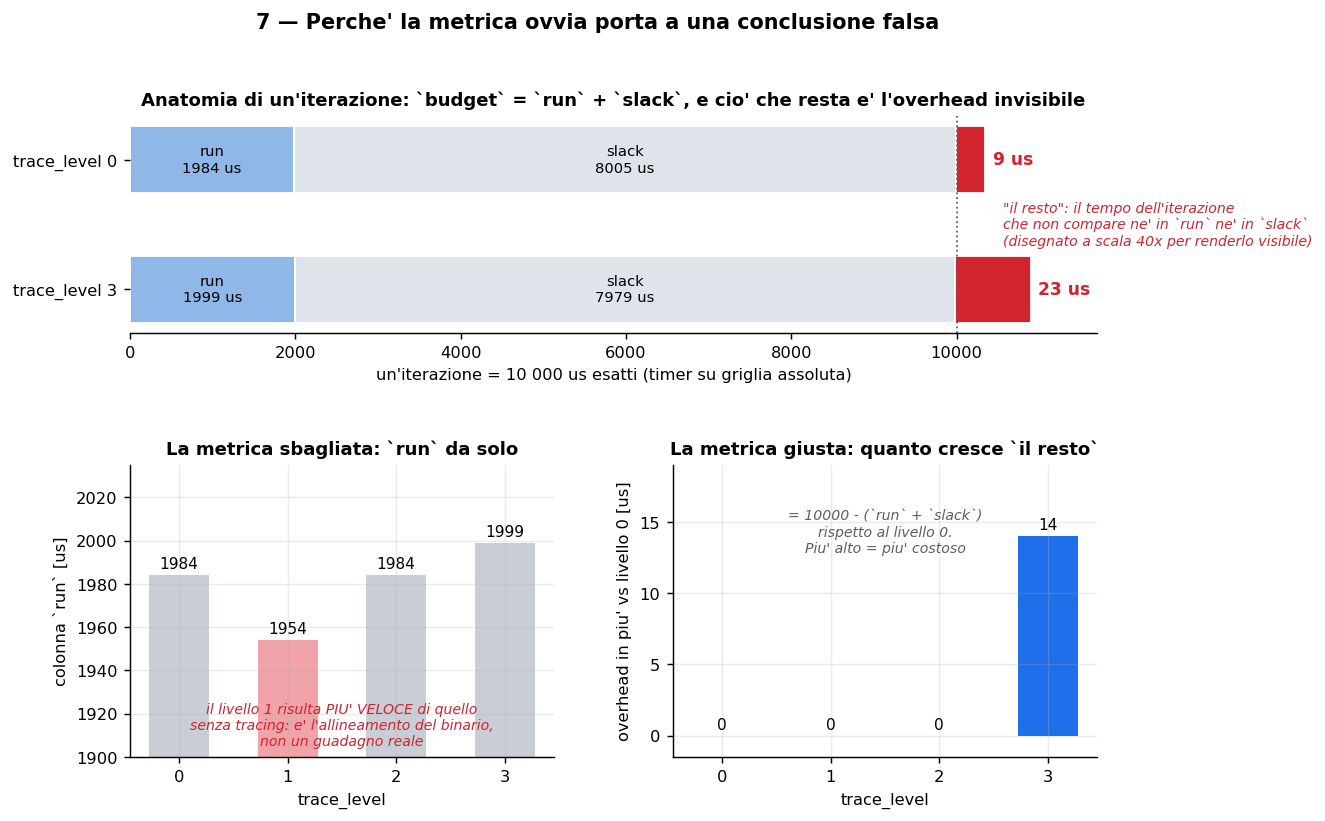
\includegraphics[width=\textwidth]{../2-DoE/figures/07_metric_artifact.png}
\caption{Anatomia di un'iterazione e confronto fra la grandezza riportata nativamente e quella
effettivamente indicativa del costo.}
\label{fig:07}
\end{figure}

La spiegazione richiede di guardare come si compone un'iterazione, riportata nel riquadro
superiore. Poich\'e il task critico si attiva su una griglia temporale fissa, fra due attivazioni
consecutive trascorrono esattamente 10\,000\us. Tale intervallo si ripartisce in tre contributi:

\begin{itemize}
\item la \textbf{fase di lavoro}, l'unica cronometrata esplicitamente;
\item il \textbf{margine residuo} rispetto alla scadenza, misurato al termine del lavoro;
\item la parte \textbf{non contabilizzata}, differenza fra il periodo e la somma delle due
precedenti, che comprende la latenza di risveglio, la scrittura del log e --- questo \`e il punto ---
la creazione e la chiusura degli elementi di traccia, che avvengono al di fuori della finestra
cronometrata.
\end{itemize}

Definiamo \emph{budget} la somma dei primi due contributi, cio\`e la porzione di iterazione che il
generatore misura. L'overhead della telemetria non compare in essa, ma nella terza: quanto pi\`u la
strumentazione lavora, tanto pi\`u il budget si riduce. L'ordinata del riquadro in basso a destra
riporta perci\`o di quanto cresce la parte non contabilizzata rispetto alla condizione senza
tracciamento.

\begin{table}[h]\centering\small
\begin{tabular}{cccccc}
\toprule
\textbf{livello} & fase di lavoro & margine residuo & \textbf{budget} & periodo & non contabilizzato \\
\midrule
0 & 1984 & 8005 & 9991 & 10\,000 & 9 \\
1 & 1954 & 8036 & 9991 & 10\,000 & 9 \\
2 & 1984 & 8006 & 9991 & 10\,000 & 9 \\
3 & 1999 & 7979 & 9977 & 10\,000 & \textbf{23} \\
\bottomrule
\end{tabular}
\caption{Scomposizione dell'iterazione per livello di tracciamento; valori in microsecondi,
mediane su 20 ripetizioni.}
\label{tab:anatomia}
\end{table}

La riga del livello~1 chiarisce l'artefatto. La fase di lavoro \emph{diminuisce} di 30\us{} rispetto
al livello 0, ma il margine residuo \emph{aumenta} di 31: i due si compensano e il budget resta
invariato. Se quei 30\us{} fossero stati lavoro realmente risparmiato, l'iterazione sarebbe
terminata prima e il margine sarebbe rimasto pi\`u ampio. Il tempo \`e semplicemente stato
contabilizzato altrove: eseguibili diversi dispongono il codice in memoria in modo leggermente
diverso, e la differenza di allineamento vale circa 30\us, cio\`e \textbf{pi\`u del segnale da
misurare}. Lo stesso vale per il periodo riportato, che al livello 3 risulta addirittura
\emph{pi\`u breve} proprio dove l'overhead cresce.

\textbf{Risultato.} Adottando il budget come variabile di risposta, i livelli 1 e 2 non producono
alcun effetto misurabile, mentre il livello 3 costa \textbf{circa 14\us{} per iterazione}: lo
0.14\,\% del periodo, ma lo 0.7\,\% del lavoro utile. Non si registra alcuna scadenza mancata a
nessun livello. La periodicit\`a non viene degradata: l'intervallo fra attivazioni consecutive resta
di 10\,000\us{} in tutte le condizioni.

\`E utile precisare che cosa \emph{non} rientra in quei 14\us. Scomponendo la parte non
contabilizzata mediante la latenza di risveglio, che il generatore registra separatamente, si
ottiene un contributo costante di circa 7.4\us{} dovuto al risveglio del thread e non attribuibile
alla telemetria; i restanti 14\us{} rappresentano il costo di \emph{costruire} gli elementi di
traccia, non di trasmetterli. La trasmissione, in questa configurazione, \`e a carico di un thread
separato: il suo costo emerger\`a nell'Esperimento 3.

\subsection{Esperimento 2: il campionamento non distingue le criticit\`a}

\`E il risultato centrale dello studio.

\begin{figure}[h]\centering
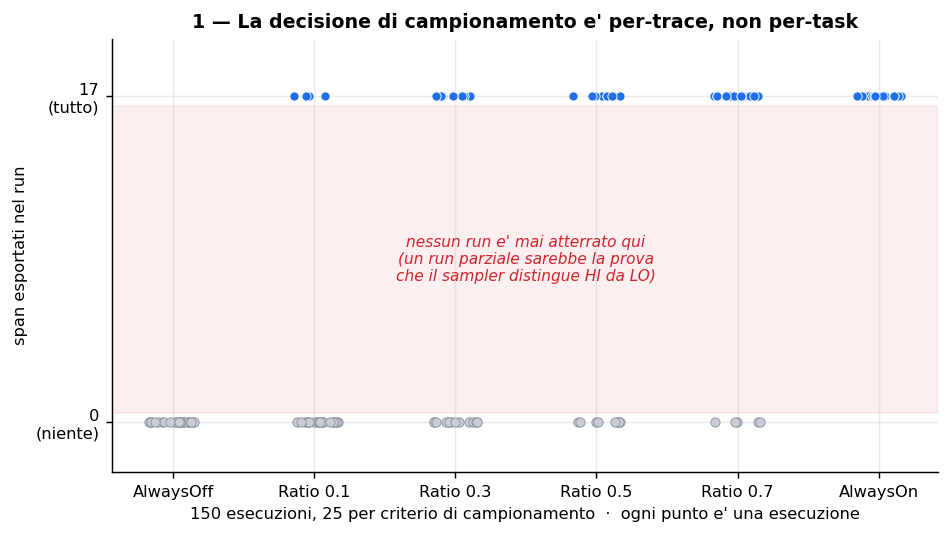
\includegraphics[width=\textwidth]{../2-DoE/figures/01_all_or_nothing.png}
\caption{Elementi di traccia emessi in ciascuna delle 150 esecuzioni, per criterio di
campionamento. La banda evidenziata copre tutti i valori intermedi.}
\label{fig:01}
\end{figure}

Nella Figura~\ref{fig:01} ogni punto rappresenta un'esecuzione. I punti si dispongono su due sole
righe: nessun elemento emesso, oppure tutti e diciassette. \textbf{La banda intermedia \`e vuota in
tutte e sei le configurazioni}: non esiste una singola esecuzione, su 150, in cui siano stati
conservati gli elementi del task critico e scartati quelli dei task di disturbo, o viceversa.

Quando un'esecuzione viene campionata, gli elementi emessi sono sempre esattamente uno per il task
critico e quattro per i task di disturbo. La ragione risiede nella struttura delle tracce: tutti i
thread vengono creati come discendenti di un unico elemento radice che rappresenta l'esecuzione, e
condividono di conseguenza il medesimo identificativo di traccia. Il criterio di campionamento
proporzionale decide in funzione di tale identificativo, e la decisione viene quindi presa
\textbf{una volta per esecuzione}, non per singolo elemento n\'e per task.

\begin{figure}[h]\centering
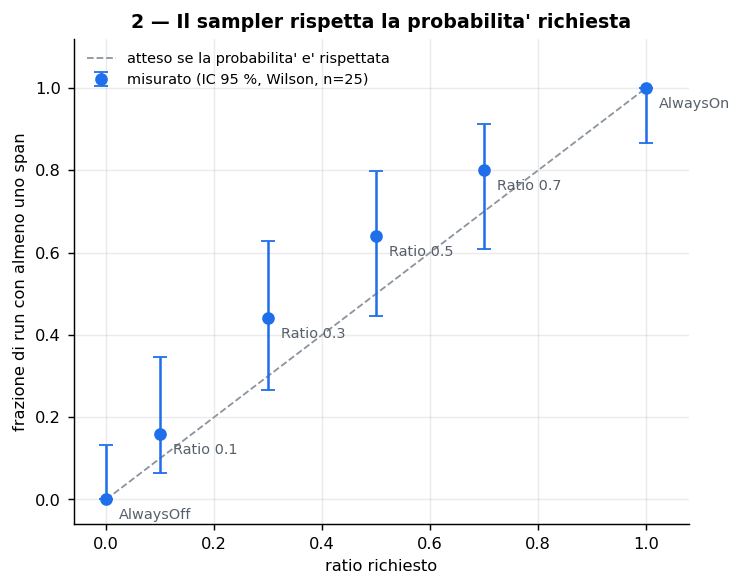
\includegraphics[width=0.62\textwidth]{../2-DoE/figures/02_sampling_fraction.png}
\caption{Frazione di esecuzioni campionate in funzione della proporzione richiesta; barre di
incertezza al 95\,\% su 25 ripetizioni per configurazione.}
\label{fig:02}
\end{figure}

La Figura~\ref{fig:02} completa il quadro e va letta insieme alla precedente. La frazione di
esecuzioni effettivamente campionate segue fedelmente la proporzione richiesta, e ogni intervallo
di confidenza contiene il valore nominale. Il meccanismo, dunque, \textbf{funziona correttamente};
ci\`o che non \`e adeguato \`e la granularit\`a alla quale opera.

\textbf{Conseguenza operativa.} Impostare una proporzione di campionamento pari a 0.1 non significa
``conserva il 10\,\% degli elementi'': significa ``scarta l'intera esecuzione, task critico
compreso, con probabilit\`a del 90\,\%''. Nei nostri dati, a tale proporzione, in 21 esecuzioni su
25 \textbf{non esiste alcuna traccia del task critico}. In un sistema a criticit\`a mista questo \`e
il comportamento meno desiderabile fra quelli possibili: la riduzione del volume di telemetria,
che \`e un'esigenza legittima, si ottiene sacrificando in modo indiscriminato proprio le
informazioni che si vorrebbero preservare. \`E la constatazione da cui muove la proposta esposta
nella \S6.

Sul piano temporale, l'esperimento non evidenzia differenze: il budget per iterazione risulta pari
a 9991\us{} in tutte e sei le configurazioni, campionamento disattivato compreso. Il confronto pi\`u
pulito \`e interno alle configurazioni proporzionali, dove le esecuzioni si dividono in campionate
e scartate in base al solo esito del sorteggio, a parit\`a di eseguibile e configurazione: i due
gruppi presentano lo stesso budget mediano, con differenza nulla entro la risoluzione della misura.

\subsection{Esperimento 3: la modalit\`a di consegna determina il costo}

\begin{figure}[h]\centering
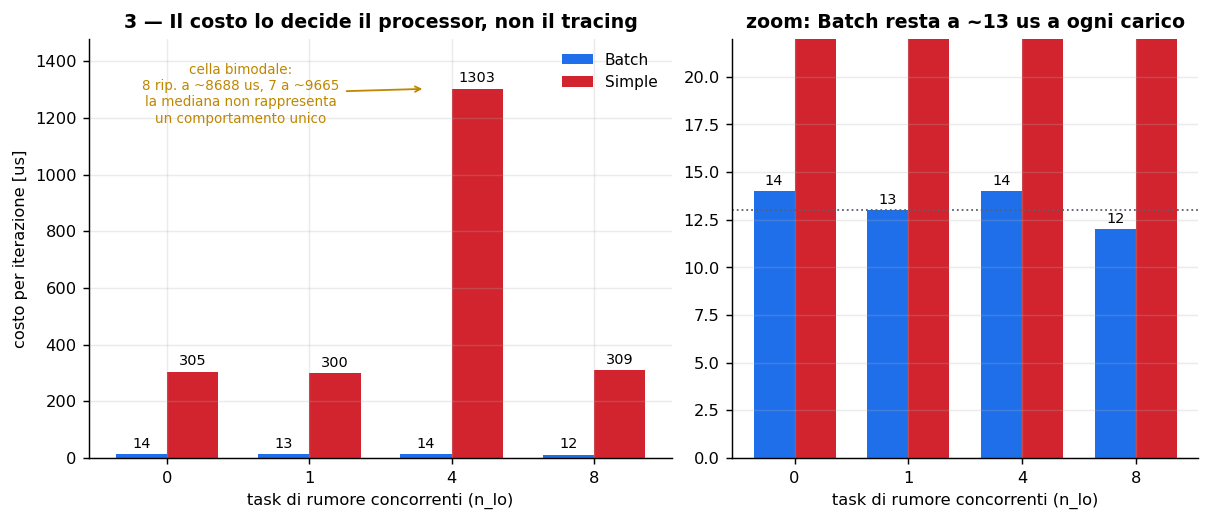
\includegraphics[width=\textwidth]{../2-DoE/figures/03_overhead_processor.png}
\caption{Costo per iterazione a carico crescente, rispetto alla condizione di controllo senza
tracciamento. A destra la stessa grandezza con scala espansa.}
\label{fig:03}
\end{figure}

La Figura~\ref{fig:03} riporta il costo per iterazione delle due modalit\`a di consegna, misurato
rispetto alla condizione di controllo allo stesso livello di carico. La consegna differita si
mantiene stabile fra 12 e 14\us{} a ogni livello di carico, in accordo con il valore ottenuto
nell'Esperimento 1. La consegna immediata costa circa \textbf{300\us}: ventitr\'e volte tanto, pari
al 3\,\% del periodo e al \textbf{15\,\% del lavoro utile}.

Il risultato sposta il baricentro delle conclusioni: non \`e la \emph{quantit\`a} di telemetria a
determinare il costo, ma il \emph{modo} in cui viene consegnata. A parit\`a di granularit\`a
massima, e quindi di numero di elementi prodotti, il costo per il task critico varia di oltre un
ordine di grandezza a seconda di questa sola scelta.

\emph{Un'avvertenza sulla lettura della figura.} La barra relativa a quattro task di disturbo
riporta un valore di 1303\us, segnalato nella figura stessa: quella configurazione presenta un
comportamento bimodale, con otto ripetizioni raggruppate attorno a un valore e sette attorno a un
altro, e la mediana cade sul primo gruppo. Il valore non va quindi interpretato come un costo
maggiore a quel livello di carico, e la non monotonia rispetto agli otto task di disturbo \`e solo
apparente. Il costo attribuibile alla consegna immediata resta quello indicato di circa 300\us;
l'origine del secondo comportamento non \`e stata determinata ed \`e segnalata fra i limiti dello
studio.

\begin{figure}[h]\centering
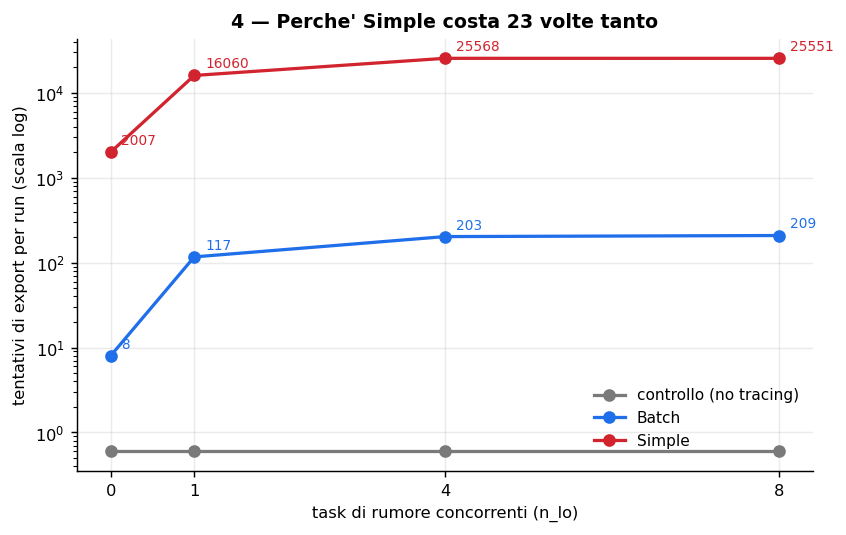
\includegraphics[width=0.72\textwidth]{../2-DoE/figures/04_export_attempts.png}
\caption{Numero di tentativi di trasmissione per esecuzione, in scala logaritmica.}
\label{fig:04}
\end{figure}

La Figura~\ref{fig:04} individua il meccanismo all'origine di tale divario, e non ne \`e una
semplice riformulazione. Nella modalit\`a immediata la trasmissione avviene \textbf{in modo sincrono,
all'interno del thread che ha appena prodotto l'elemento}, sotto un blocco condiviso fra tutti i
thread; nella modalit\`a differita gli elementi vengono accodati e trasmessi da un thread dedicato
a intervalli regolari. Il numero di tentativi di trasmissione per esecuzione passa da circa 230 a
oltre 25\,000: il task critico, nella prima modalit\`a, sostiene di persona il costo di ogni singola
trasmissione e concorre per il blocco condiviso con tutti gli altri thread.

Va sottolineato che nelle esecuzioni in esame \textbf{nessun servizio di raccolta era in ascolto}:
i tentativi di trasmissione falliscono immediatamente. Questa \`e la condizione \emph{pi\`u
favorevole} alla modalit\`a immediata; con un servizio realmente attivo, che accetta la connessione
e risponde, il divario sarebbe maggiore. I valori riportati vanno quindi intesi come un limite
inferiore.

\begin{figure}[h]\centering
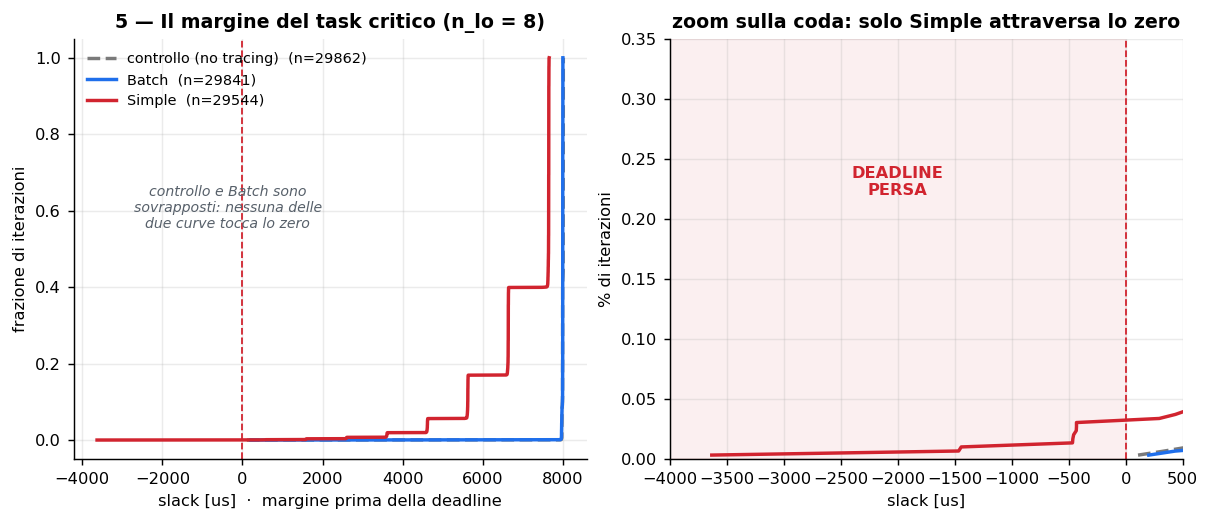
\includegraphics[width=\textwidth]{../2-DoE/figures/05_slack_distribution.png}
\caption{Distribuzione cumulativa del margine residuo del task critico al carico massimo; a destra
l'ingrandimento della coda.}
\label{fig:05}
\end{figure}

La Figura~\ref{fig:05} riporta la conseguenza sul rispetto delle scadenze. La condizione di
controllo e quella a consegna differita risultano sovrapposte e \textbf{non raggiungono mai lo
zero}: ogni iterazione si conclude con almeno 65\us{} di margine. La consegna immediata presenta
invece una coda che attraversa lo zero.

\`E l'unica figura che mostri il \emph{margine} anzich\'e il semplice conteggio dei fallimenti, e la
distinzione \`e sostanziale. Nove scadenze mancate su circa 29\,500 iterazioni (lo 0.03\,\%)
potrebbero apparire trascurabili in forma tabellare; la distribuzione mostra invece che il
comportamento \`e \textbf{qualitativamente diverso}, con una coda che si estende fino a
$-3631$\us: il task critico non sfora occasionalmente di poco, ma pu\`o eccedere la propria
scadenza di oltre un terzo del periodo. Si osserva inoltre che la separazione fra le due modalit\`a
\`e netta e priva di sovrapposizione, per cui la conclusione non dipende dalla scelta di una soglia.

Complessivamente, sulle 180 esecuzioni dell'esperimento le scadenze mancate sono 21, tutte nella
modalit\`a a consegna immediata e in presenza di carico concorrente; le condizioni di controllo e
quelle a consegna differita ne registrano \textbf{zero a qualunque livello di carico}. Le scadenze
mancate risultano distribuite uniformemente lungo l'esecuzione, e non concentrate in prossimit\`a
del termine: non sono quindi riconducibili alla fase di chiusura del programma.

Un'ulteriore osservazione riguarda la robustezza. Nella modalit\`a a consegna immediata, in presenza
di pi\`u thread, una frazione rilevante delle esecuzioni termina in modo anomalo al momento della
chiusura, con probabilit\`a crescente al crescere del numero di thread. Il fenomeno ha origine
nell'interazione fra il modo in cui il generatore di carico termina i propri thread e il fatto che
la funzione di consegna immediata sia dichiarata come non sollevante eccezioni: la terminazione
attraversa tale funzione e provoca l'arresto del processo. L'anomalia si manifesta \emph{dopo} che
tutti i dati sono stati scritti, e non compromette quindi le misure; \`e per\`o rilevante in
prospettiva applicativa, poich\'e in questa configurazione la scelta della modalit\`a di consegna
non degrada soltanto le prestazioni del task critico, ma pu\`o determinarne la terminazione.

\subsection{Sintesi dei risultati}

\begin{table}[h]\centering\small
\begin{tabular}{p{6.4cm}p{8.2cm}}
\toprule
\textbf{domanda} & \textbf{risposta sperimentale} \\
\midrule
La pipeline di telemetria prioritizza i task critici? &
\textbf{No.} La decisione di campionamento \`e presa per traccia e non per task: zero esecuzioni
parziali su 150. Ridurre il volume significa perdere anche il task critico. \\
\addlinespace
Quanto costa il monitoraggio al task critico? &
Circa 14\us{} per iterazione con consegna differita, a qualunque livello di carico; circa 300\us{}
con consegna immediata, pari al 15\,\% del lavoro utile. \\
\addlinespace
Il monitoraggio compromette il rispetto delle scadenze? &
Solo con consegna immediata e carico concorrente: 21 scadenze mancate, con margini fino a
$-3631$\us. Con consegna differita, nessuna. \\
\addlinespace
La granularit\`a del tracciamento \`e il fattore determinante? &
No: incide per 14\us{} soltanto al livello massimo. Il fattore determinante \`e la modalit\`a di
consegna. \\
\bottomrule
\end{tabular}
\caption{Sintesi delle evidenze raccolte.}
\end{table}

\subsection{Limiti dello studio}

\textbf{Assenza di un servizio di raccolta.} Tutte le esecuzioni sono state condotte senza un
servizio in ascolto. Come osservato, ci\`o rende i costi misurati un limite inferiore.

\textbf{Configurazione con comportamento bimodale.} Una delle dodici configurazioni
dell'Esperimento 3 presenta due comportamenti distinti fra le ripetizioni, per i quali non \`e stata
individuata una spiegazione; il dato \`e stato riportato con l'avvertenza corrispondente anzich\'e
essere sintetizzato in un valore unico.

\textbf{Piattaforma singola.} Le misure provengono da un solo sistema, con quattro core fisici e un
inviluppo termico limitato. I valori assoluti non sono trasferibili ad altro hardware; i confronti
fra configurazioni, condotti a parit\`a di ogni altra condizione, lo sono.

\section{Proposta: un criterio di campionamento consapevole della criticit\`a}

I risultati dell'Esperimento 2 individuano un limite preciso e circoscritto: il criterio di
campionamento proporzionale opera sull'identificativo di traccia, e poich\'e tutti i thread di
un'esecuzione condividono tale identificativo, la decisione ricade sull'intera esecuzione. Non
esiste, con i componenti disponibili, un modo di esprimere una politica del tipo ``conserva sempre
le tracce dei task critici e riduci quelle dei task best-effort''.

In questa sezione delineiamo come tale limite possa essere superato. L'esposizione resta a livello
di progetto: si indicano i punti del sistema su cui intervenire e la logica da introdurvi, senza
scendere nel dettaglio implementativo.

\subsection{Il vincolo da cui partire}

L'analisi del funzionamento della libreria evidenzia due elementi che condizionano qualunque
soluzione.

\textbf{Il momento della decisione.} Il componente che decide se registrare una traccia viene
interpellato \emph{all'atto della creazione} dell'elemento, e riceve il nome dell'elemento e i soli
attributi passati contestualmente alla creazione. Nel codice a disposizione, gli attributi che
descrivono la politica di scheduling e la priorit\`a --- cio\`e proprio le informazioni che
identificano la criticit\`a di un task --- vengono impostati \emph{successivamente}. Un criterio
personalizzato, allo stato attuale, non li vedrebbe.

\textbf{La struttura delle tracce.} Ogni thread viene creato come discendente dell'elemento radice
che rappresenta l'esecuzione. Questa scelta \`e ci\`o che rende l'intera esecuzione una traccia sola,
ed \`e la causa diretta del comportamento osservato in Figura~\ref{fig:01}.

\subsection{Due interventi complementari}

\textbf{Primo intervento: rendere la criticit\`a visibile al momento della decisione.} Sono
possibili due strade, di costo diverso. La meno invasiva consiste nell'adottare una convenzione sui
nomi dei task, che il criterio personalizzato pu\`o esaminare: il nome dell'elemento \`e infatti
gi\`a disponibile al momento della decisione. Le configurazioni della campagna adottano gi\`a nomi
distinti per i task critici e per quelli di disturbo, per cui questa strada non richiederebbe
modifiche al codice esistente. La strada pi\`u pulita, ma che comporta una piccola modifica nel
punto in cui gli elementi dei thread vengono creati, consiste nel passare la criticit\`a come
attributo contestualmente alla creazione, anzich\'e subito dopo. \`E preferibile in prospettiva,
perch\'e non lega la politica a una convenzione sui nomi.

\textbf{Secondo intervento: separare le tracce per criticit\`a.} \`E il punto essenziale, e senza
di esso il primo non basta. Finch\'e tutti i thread appartengono alla stessa traccia, qualunque
criterio proporzionale continuer\`a a valutare un unico identificativo, e le decisioni sui diversi
task resteranno rigidamente accoppiate. Occorre che \emph{ciascun thread avvii una propria traccia},
cos\`i che ogni criticit\`a possa essere campionata in modo indipendente.

La relazione causale con l'esecuzione principale, che ha valore diagnostico e non va perduta, pu\`o
essere mantenuta sostituendo il legame di discendenza con un \emph{collegamento} fra tracce, che la
libreria prevede proprio per correlare tracce distinte. Il risultato \`e che le tracce restano
navigabili come oggi, ma diventano campionabili separatamente.

\subsection{Dove intervenire}

Gli interventi si concentrano in tre punti, tutti circoscritti.

\begin{enumerate}
\item \textbf{Un nuovo componente di campionamento}, da introdurre come file a s\'e stante. Ne
implementerebbe l'interfaccia prevista dalla libreria, esponendo una decisione basata sulla
criticit\`a riconosciuta: conservare sempre gli elementi dei task critici, applicare una
proporzione configurabile agli altri, ed ereditare la decisione del genitore per gli elementi
discendenti, cos\`i che una traccia campionata resti completa.

\item \textbf{La funzione di inizializzazione del tracciamento}, dove il fornitore di tracce viene
costruito e dove viene scelto il criterio di campionamento. \`E il punto in cui il nuovo componente
verrebbe registrato, affiancandolo a quelli esistenti secondo lo stesso schema gi\`a utilizzato per
gli altri parametri di configurazione, in modo che la scelta resti selezionabile e non sostitutiva.

\item \textbf{Il punto di creazione degli elementi associati ai thread}, per i due aspetti discussi
sopra: rendere disponibile la criticit\`a al momento della decisione e avviare una traccia distinta
per thread mantenendo il collegamento con l'esecuzione principale.
\end{enumerate}

\subsection{Come verificarne l'efficacia}

La proposta \`e verificabile con la stessa impostazione sperimentale gi\`a costruita, il che ne
rende la valutazione immediata. Sarebbe sufficiente ripetere l'Esperimento 2 sostituendo il criterio
di campionamento, e osservare la Figura~\ref{fig:01}: con un criterio consapevole della criticit\`a,
i punti dovrebbero disporsi \textbf{nella banda intermedia}, oggi vuota, con gli elementi del task
critico sempre presenti e quelli dei task di disturbo ridotti secondo la proporzione impostata.
La stessa figura che oggi documenta il limite diventerebbe quindi la verifica del suo superamento.

Andrebbe inoltre misurato, con l'impostazione dell'Esperimento 1, il costo del nuovo criterio: la
decisione viene presa a ogni creazione di elemento, e un criterio che esamini attributi o nomi \`e
pi\`u oneroso di uno che valuti un solo identificativo. L'ordine di grandezza atteso \`e tale da non
incidere in modo apprezzabile, ma trattandosi di un sistema real-time la verifica \`e necessaria e
non pu\`o essere data per acquisita.

\subsection{Osservazione conclusiva}

Vale la pena rilevare che i due risultati principali di questo studio indicano due margini di
intervento di natura diversa. Il costo di \emph{costruire} gli elementi di traccia --- circa 14\us{}
per iterazione --- \`e sostenuto necessariamente dal thread che li genera e non \`e eliminabile per
via architetturale. Il costo di \emph{consegnarli}, che come si \`e visto \`e di gran lunga
superiore, \`e invece \emph{collocabile}: la modalit\`a differita lo sposta su un thread di
servizio, sottraendolo al percorso critico. La proposta qui delineata agisce su un terzo asse, il
\emph{volume} della telemetria, rendendone la riduzione selettiva anzich\'e indiscriminata.

Le tre leve sono indipendenti e componibili. Per un sistema a criticit\`a mista, le evidenze
raccolte suggeriscono di adottare la consegna differita, di non affidare al campionamento
proporzionale la protezione dei task critici, e di introdurre un criterio in grado di distinguerli.

\end{document}
